\section{Динамические массивы (переменной длины). Операции над массивами: поиск, вставка, удаление}
\section{Многомерные массивы - подходы к реализации}
\section{Связанные (linked) структуры данных}
\section{Динамические структуры данных: простой линейный список. Основные операции: поиск, вставка, удаление}
\textbf{Линейный список} -- это динамическая структура данных, каждый элемент которой посредством указателя связывается со следующим элементом.

\textbf{Односвязный список} -- это простейшая реализация списка. В узлах хранятся данные и указатель на следующий элемент в списке.

Базовые операции на списке:
\begin{itemize}
    \item
          \textbf{Вставка}

          Для вставки обычно создается новый узел, в него устанавливается указатель на старый головной узел (\textit{head node}), после этого в переменную головы списка устанавливается указатель на новый узел.
    \item
          \textbf{Поиск}

          Для того, чтобы найти элемент по значению, будем двигаться по списку от головы до конца и сравнивать значение в элементах с искомым. Если элемента в списке нет, то возвращаем \mverb{NULL}.
    \item
          \textbf{Удаление}

          Для того, чтобы удалить голову списка, переназначим указатель на голову на второй элемент списка, а голову удалим.

          Удаление элемента после заданного происходит следующим образом: изменим ссылку на следующий элемент на следующий за удаляемым, затем удалим нужный объект.
\end{itemize}

Реализация односвязного списка:
\begin{minted}{C++}
// List1.h
#ifndef _LIST1_INCLUDED_

#define _LIST1_INCLUDED_ 1

//#include <stdlib.h>
#include <cstddef>

#define	ITEMS_LIMIT	1000000

class CListItem {
private:
	int m_nValue;
	CListItem* m_pLink;
public:
	CListItem( int nValue = 0) { m_nValue = nValue; m_pLink = nullptr; };
	~CListItem() {};
	int GetValue( void) { return m_nValue; };
	CListItem* GetLink( void) { return m_pLink; };
	void SetLink( CListItem* pNewLink) { m_pLink = pNewLink; };
	void Print( void);
};

class CList {
private:
	CListItem* m_pHead;
	size_t m_nItemsCount;
	size_t m_nItemsLimit;
public:
	CList( size_t nItemsLimit = 0);
	~CList();
	size_t GetItemsCount(void) { return m_nItemsCount; }
	size_t GetItemsLimit(void) { return m_nItemsLimit; }
	bool Insert( CListItem* pNewItem, CListItem* pPosition = nullptr);
	bool Enumerate( CListItem** ppListItem);
	CListItem* Find( int nSample);
	void Purge( void);
//	bool Extract( )
	void Print( void);
};

#endif //_LIST1_INCLUDED_

// List1.cpp
#include "List1.h"

#include <iostream>

/*--             --
- Class CListItem -
--             --*/

void CListItem::Print(void)
{
    std::cout << "Item value: " << m_nValue << "\n";
    return;
}

/*--                                                     --
- Class CList                                             -
- !! The class methods are not re-entry- and thread-safe! -
--                                                     --*/

CList::CList(size_t nItemsLimit)
{
    m_pHead = nullptr;
    m_nItemsCount = 0;
    m_nItemsLimit = ((nItemsLimit > 0) && (nItemsLimit <= ITEMS_LIMIT))
                        ? nItemsLimit
                        : ITEMS_LIMIT;
    return;
}

CList::~CList()
{
    Purge();
    return;
}

bool CList::Insert(CListItem* pNewItem, CListItem* pPosition)
{
    if ((pNewItem == nullptr) || (m_nItemsCount >= m_nItemsLimit))
        return false;
    if (pPosition != nullptr)
    {  // insertion position is pointed
        pNewItem->SetLink(pPosition->GetLink());
        pPosition->SetLink(pNewItem);
    }
    else
    {  // use any suitable location
        pNewItem->SetLink(m_pHead);
        m_pHead = pNewItem;  // add to head of the list (fastest)
    }
    ++m_nItemsCount;
    return true;
}

bool CList::Enumerate(CListItem** ppListItem)
{
    if (ppListItem == nullptr)
        return false;
    if (*ppListItem == nullptr)  // starting enumeration
        *ppListItem = m_pHead;
    else  // continuing enumeration
        *ppListItem = (*ppListItem)->GetLink();
    return (*ppListItem != nullptr) ? true : false;
}

CListItem* CList::Find(int nSample)
{
    CListItem* pDesiredItem = nullptr;
    for (CListItem* pItem = nullptr; Enumerate(&pItem);)
    {
        if (pItem->GetValue() == nSample)
        {
            pDesiredItem = pItem;
            break;
        }
        else
            continue;
    }
    return pDesiredItem;
}

void CList::Purge(void)
{
    for (CListItem* pItem = nullptr; Enumerate(&pItem);)
        delete pItem;
    m_pHead = nullptr;
    m_nItemsCount = 0;
    return;
}

void CList::Print(void)
{
    std::cout << "Items in the list: " << m_nItemsCount << "\n";
    for (CListItem* pItem = nullptr; Enumerate(&pItem);)
        pItem->Print();
    return;
}
\end{minted}

\textbf{Полезные ссылки:}
\begin{itemize}
    \item \href{https://drive.google.com/drive/folders/1EClc2YdBxoKuk4g1VPfmMlzmHIsJwC35}{Google Drive - материалы ОАиП 2 семестр}
    \item \href{https://learn.microsoft.com/ru-ru/cpp/cpp/arrays-cpp?view=msvc-170}{Microsoft Learn - Массивы (C++)}
    \item \href{https://neerc.ifmo.ru/wiki/index.php?title=%D0%A1%D0%BF%D0%B8%D1%81%D0%BE%D0%BA}{ИТМО Wiki - Список}
\end{itemize}
\section{Динамические структуры данных: двунаправленный список, кольцо. Основные операции: поиск, вставка, удаление}
\subsection{Двусвязный список}

\textbf{Двусвязный список} -- это двусторонний список, в котором каждый узел имеет два указателя, следующий и предыдущий, которые ссылаются как на следующий узел, так и на предыдущий узел соответственно. В отличие от односвязного списка, где каждый узел указывает только на следующий узел, двусвязный список имеет дополнительный предыдущий указатель, который позволяет осуществлять обход как в прямом, так и в обратном направлении.

В двусвязном списке для отслеживания списка используются два указателя: head (указывающий на первый узел) и tail (указывающий на последний узел).

Двусвязный список поддерживает следующие основные операции:
\begin{itemize}
    \item Вставка элемента в произвольное место ($O(1)$);
    \item Удаление элемента ($O(1)$, если известно, где он находится и $O(n)$, если его сперва надой найти);
    \item Поиск элемента $O(n)$.
\end{itemize}

\begin{minted}{C++}
// C++ program to Implement doubly linked list
#include <iostream>

// Define a class named Node to represent a node in the
// doubly linked list.
class Node {
public:
  // Data part of the node.
  int data;
  // Pointer to the next node.
  Node *next;
  // Pointer to the previous node.
  Node *prev;

  // Constructor to initialize the node with given data.
  Node(int data) {
    this->data = data;
    this->next = nullptr;
    this->prev = nullptr;
  }
};

// Function to find a first node containing given value
// Returns pointer to the node if such node is present
// in the list and `nullptr` if not.
Node *find(Node *head, int value) {
  for (; head != nullptr; head = head->next) {
    if (head->data == value) {
      break;
    }
  }
  return head;
}
    
// Function to insert a node at the beginning of the doubly
// linked list.
void insertAtBeginning(Node *&head, int data) {
  // Create a new node with the given data.
  Node *newNode = new Node(data);

  // Check if the doubly linked list is empty.
  if (head == nullptr) {
    head = newNode;
    return;
  }

  // Update the next and previous pointers to insert the
  // new node at the beginning.
  newNode->next = head;
  head->prev = newNode;
  head = newNode;
}

// Function to insert a node at the end of the doubly linked
// list.
void insertAtEnd(Node *&head, int data) {
  // Create a new node with the given data.
  Node *newNode = new Node(data);

  // Check if the doubly linked list is empty.
  if (head == nullptr) {
    head = newNode;
    return;
  }

  // Traverse to the last node of the list.
  Node *temp = head;
  while (temp->next != nullptr) {
    temp = temp->next;
  }

  // Update the next and previous pointers to insert the
  // new node at the end.
  temp->next = newNode;
  newNode->prev = temp;
}

// Function to insert a node at a specified position in the
// doubly linked list.
void insertAtPosition(Node *&head, int data, int position) {
  if (position < 1) {
    std::cout << "Position should be >= 1." << std::endl;
    return;
  }

  // If inserting at the head position.
  if (position == 1) {
    insertAtBeginning(head, data);
    return;
  }

  // Create a new node with the given data.
  Node *newNode = new Node(data);
  Node *temp = head;

  // Traverse to the node before the specified position.
  for (int i = 1; temp != nullptr && i < position - 1; i++) {
    temp = temp->next;
  }

  // Check if the position is greater than the number of
  // nodes.
  if (temp == nullptr) {
    std::cout << "Position greater than the number of nodes." << std::endl;
    return;
  }

  // Update the next and previous pointers to insert the
  // new node at the specified position.
  newNode->next = temp->next;
  newNode->prev = temp;
  if (temp->next != nullptr) {
    temp->next->prev = newNode;
  }
  temp->next = newNode;
}

// Function to delete a node from the beginning of the
// doubly linked list.
void deleteAtBeginning(Node *&head) {
  // Check if the doubly linked list is empty.
  if (head == nullptr) {
    std::cout << "The list is already empty." << std::endl;
    return;
  }

  // Update the head pointer and delete the first node.
  Node *temp = head;
  head = head->next;
  if (head != nullptr) {
    head->prev = nullptr;
  }
  delete temp;
}

// Function to delete a node from the end of the doubly
// linked list.
void deleteAtEnd(Node *&head) {
  // Check if the doubly linked list is empty.
  if (head == nullptr) {
    std::cout << "The list is already empty." << std::endl;
    return;
  }

  Node *temp = head;
  // If there is only one node in the list.
  if (temp->next == nullptr) {
    head = nullptr;
    delete temp;
    return;
  }

  // Traverse to the last node of the list.
  while (temp->next != nullptr) {
    temp = temp->next;
  }

  // Update the previous pointer of the second last node
  // and delete the last node.
  temp->prev->next = nullptr;
  delete temp;
}

// Function to delete a node from a specified position in
// the doubly linked list.
void deleteAtPosition(Node *&head, int position) {
  // Check if the doubly linked list is empty.
  if (head == nullptr) {
    std::cout << "The list is already empty." << std::endl;
    return;
  }

  // If deleting the head node.
  if (position == 1) {
    deleteAtBeginning(head);
    return;
  }

  Node *temp = head;
  // Traverse to the node at the specified position.
  for (int i = 1; temp != nullptr && i < position; i++) {
    temp = temp->next;
  }

  // Check if the position is greater than the number of
  // nodes.
  if (temp == nullptr) {
    std::cout << "Position is greater than the number of "
                 "nodes."
              << std::endl;
    return;
  }

  // Update the next and previous pointers and delete the
  // node at the specified position.
  if (temp->next != nullptr) {
    temp->next->prev = temp->prev;
  }
  if (temp->prev != nullptr) {
    temp->prev->next = temp->next;
  }
  delete temp;
}

// Function to print the doubly linked list in forward
// direction.
void printListForward(Node *head) {
  Node *temp = head;
  std::cout << "Forward List: ";
  while (temp != nullptr) {
    std::cout << temp->data << " ";
    temp = temp->next;
  }
  std::cout << std::endl;
}

// Function to print the doubly linked list in reverse
// direction.
void printListReverse(Node *head) {
  Node *temp = head;
  if (temp == nullptr) {
    std::cout << "The list is empty." << std::endl;
    return;
  }

  // Move to the end of the list.
  while (temp->next != nullptr) {
    temp = temp->next;
  }

  // Traverse backwards.
  std::cout << "Reverse List: ";
  while (temp != nullptr) {
    std::cout << temp->data << " ";
    temp = temp->prev;
  }
  std::cout << std::endl;
}

int main() {
  Node *head = nullptr;

  // Demonstrating various operations on the doubly linked
  // list.
  // Insertion at End
  insertAtEnd(head, 10);
  insertAtEnd(head, 20);
  // Insertion at beginning
  insertAtBeginning(head, 5);
  // Insertion at specific position
  insertAtPosition(head, 15, 2);

  // print the list
  std::cout << "After Insertions:" << std::endl;
  printListForward(head);
  printListReverse(head);

  // deletion from beginning
  deleteAtBeginning(head);
  // deletion from end
  deleteAtEnd(head);
  // deletion from specific position
  deleteAtPosition(head, 2);

  std::cout << "After Deletions:" << std::endl;
  printListForward(head);

  return 0;
}
\end{minted}

\subsection{Кольцевой список}

\textbf{Кольцевой (циклический, замкнутый) связный список} — это разновидность связного списка, при которой первый элемент указывает на последний, а последний — на первый. Кольцевой (циклический, замкнутый) связный список можно сделать как из односвязного (однонаправленного), так и из двусвязного (двунаправленного) списка.

\textbf{Кольцевой связный список из односвязного}

В односвязном списке указатель \texttt{next} последнего узла указывает на первый узел.

\textbf{Кольцевой связный список из двусвязного}

В двусвязном списке указатель next последнего узла указывает на первый узел, а указатель \texttt{previous} первого — на последний. Так получается кольцевой связный список в обоих направлениях.

Здесь надо учитывать следующие важные моменты:
\begin{itemize}
    \item \texttt{next} последней ссылки указывает на первую ссылку списка в обоих случаях — в односвязном списке и в двусвязном.
    \item \texttt{previous} первой ссылки указывает на последнюю ссылку в двусвязном списке.
\end{itemize}

\section{Динамические структуры данных: стек. Основные операции: поиск, вставка, удаление}
\subsection{Понятие стека}
Стек~--- абстрактный тип данных, представляющий собой список элементов, организованных по принципу
LIFO (англ. last in -- first out, «последним пришёл -- первым вышел>>). Стеки могут быть построены на основе других, более фундаментальных
структурах данных, например, можно реализовать стек как обертку над массивом с указателем или на основе списка. Проще говоря, стек представляет
собой абстрактный интерфейс доступа к данным, а не конкретную структуру данных.

Организация данных по принципу LIFO означает, что элементы могут добавляться и извлекаться только с вершины стека. При этом при добавлении
элемента, именно он становится новой вершиной стека, а при удалении, вершиной становится предыдущий элемент.

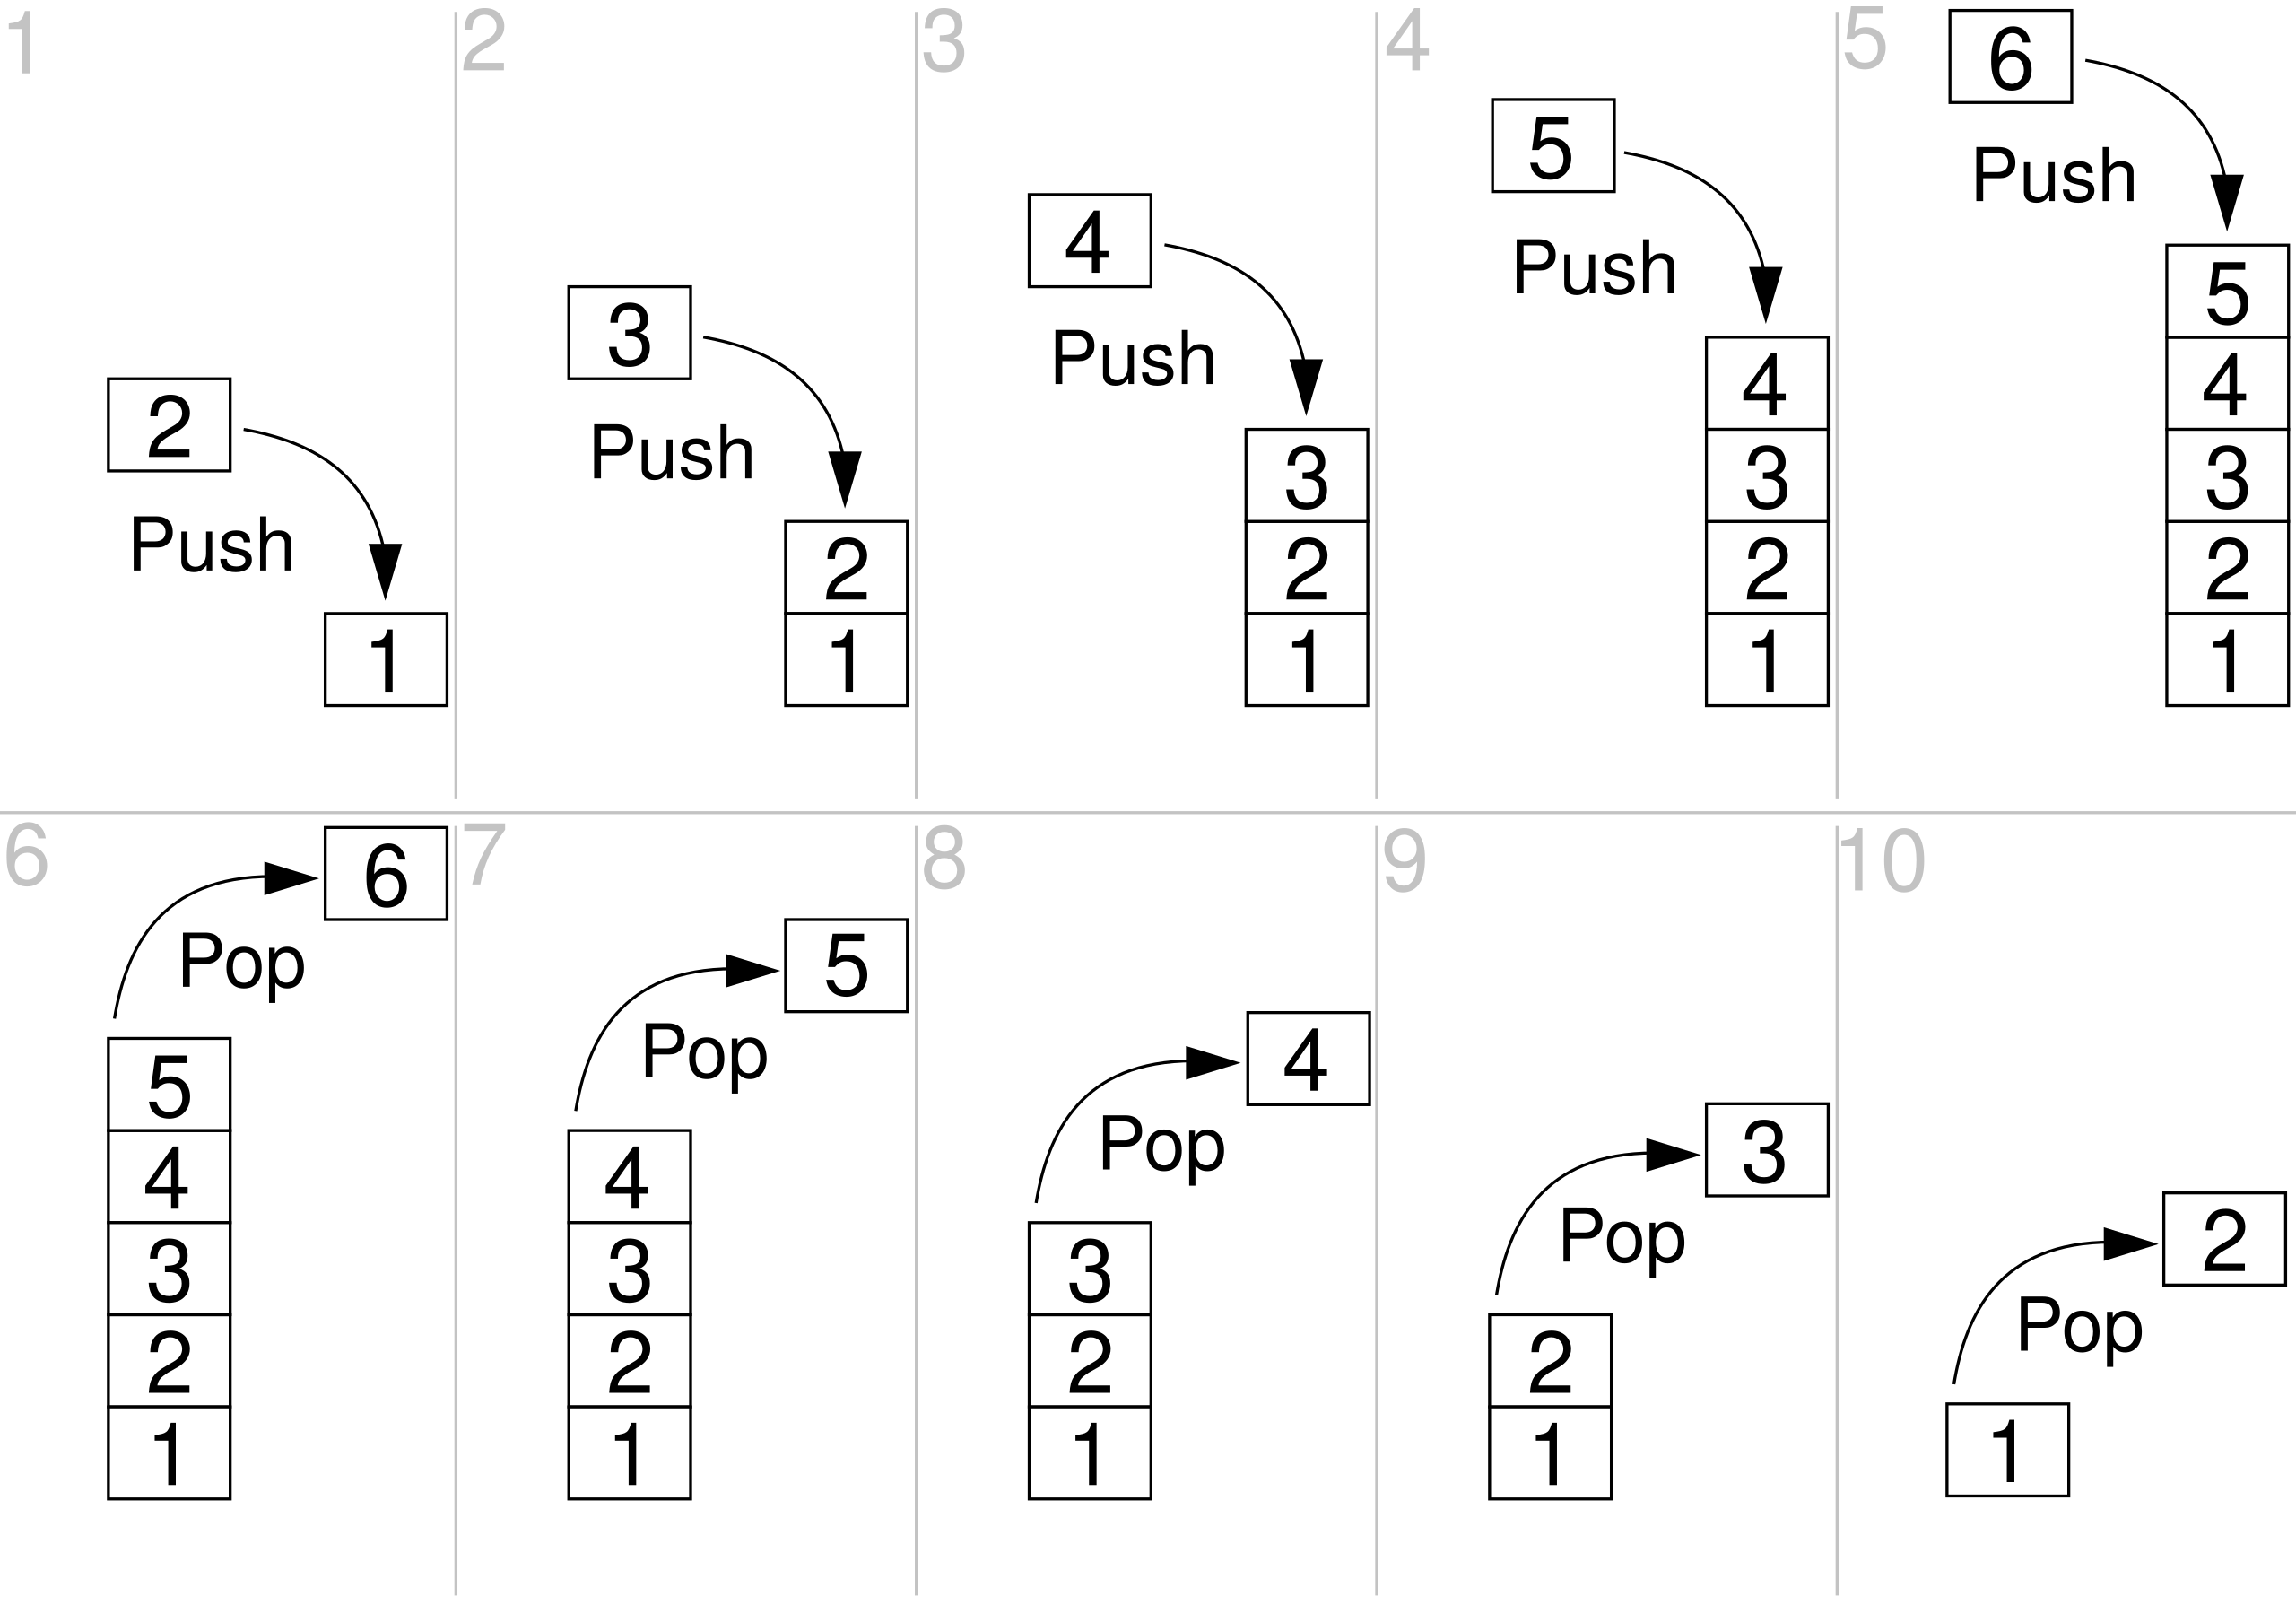
\includegraphics[width=0.9\textwidth]{resources/19-26/stack.png}

В стандартной библиотеке С++ присутствует реализация \cppref[стека]{cpp/container/stack}, объявленная в соответствующем
\cppref[заголовке]{cpp/header/stack}. Стоит отметить, что шаблон \mverb{std::stack<T>} не является
структурой данных сам по себе, а лишь предоставляет интерфейс стека поверх какой-либо другой структуры (по умолчанию, \cppref[\texttt{std::deque<T>}]{cpp/container/deque}).
Помимо этого, в качестве стека можно тривиально использовать динамический массив \cppref[\texttt{std::vector<T>}]{cpp/container/vector} с его
методами \mverb{push_back(T &&)}, \mverb{back()} и \mverb{pop_back()}.
\subsection{Операции над стеком}
Когда речь идет о стеке, подразумевается структура данных со следующими операциями:
\begin{enumerate}
  \item Добавить элемент в верхушку стека (\mverb{push()}).
  \item Удалить элемент из верхушки стека (\mverb{pop()}).
  \item Найти элемент в стеке.
\end{enumerate}

Часто также требуется поддержка операции чтения вершины без ее удаления (\mverb{peek()}, также \mverb{top()}) и
проверки на пустоту (\mverb{empty()}). В эффективной реализации все вышеназванные операции, кроме поиска, имеют временную сложность
\(O(1)\). Поиск имеет сложность $O(n)$.

\subsection{Пример реализации стека}
Приведем реализацию стека (С++ 11) на основе статического массива фиксированной длины. Данная реализация будет использовать шаблоны и
\cppref[\texttt{assert(bool)}]{cpp/error/assert} для проверок инвариантов.

\begin{minted}{C++}
template <typename T, size_t N> class Stack {
public:
  Stack() = default;
  ~Stack() = default;

  bool empty() const { return count_ == 0; }
  size_t capacity() const { return N; }
  size_t count() const { return count_; }

  const T &Peek() const {
    assert(count_ > 0 && "Stack is empty.");
    return data_[count_ - 1];
  }
  T &Peek() {
    assert(count_ > 0 && "Stack is empty.");
    return data_[count_ - 1];
  }

  T Pop() {
    assert(count_ > 0 && "Stack is empty.");
    --count_;
    return data_[count_];
  }
  void Push(const T &item) {
    assert(count_ < N && "Stack is full.");
    data_[count_] = item;
    ++count_;
  }
  void Push(T &&item) {
    assert(count_ < N && "Stack is full.");
    data_[count_] = item;
    ++count_;
  }
  T* Find(const T& item) {
    for (size_t i = 0; i < count_; ++i) {
      if (data_[i] == item) {
        return &data_[i];
      }
    }
    return nullptr;
  }

  T *begin() { return data_; }
  T *end() { return data_ + count_; }
  const T *begin() const { return data_; }
  const T *end() const { return data_ + count_; }

private:
  T data_[N];
  size_t count_{};
};
\end{minted}
\section{Динамические структуры данных: очередь. Основные операции: поиск, вставка, удаление}
Очередь~--- абстрактный тип данных, представляющий собой список данных, организованных по принципу FIFO (англ. first in -- first out, <<первым пришел первым вышел>>).
Очереди могут быть построены на основе других, более фундаментальных структурах данных. Например, очередь может быть внутренне реализована как
список. Об очереди можно судить скорее как об интерфейсе доступа к данным.

Организация по принципу FIFO означает, что элементы могут извлекаться с одного конца (головы), а добавляться~--- с другого (хвоста).

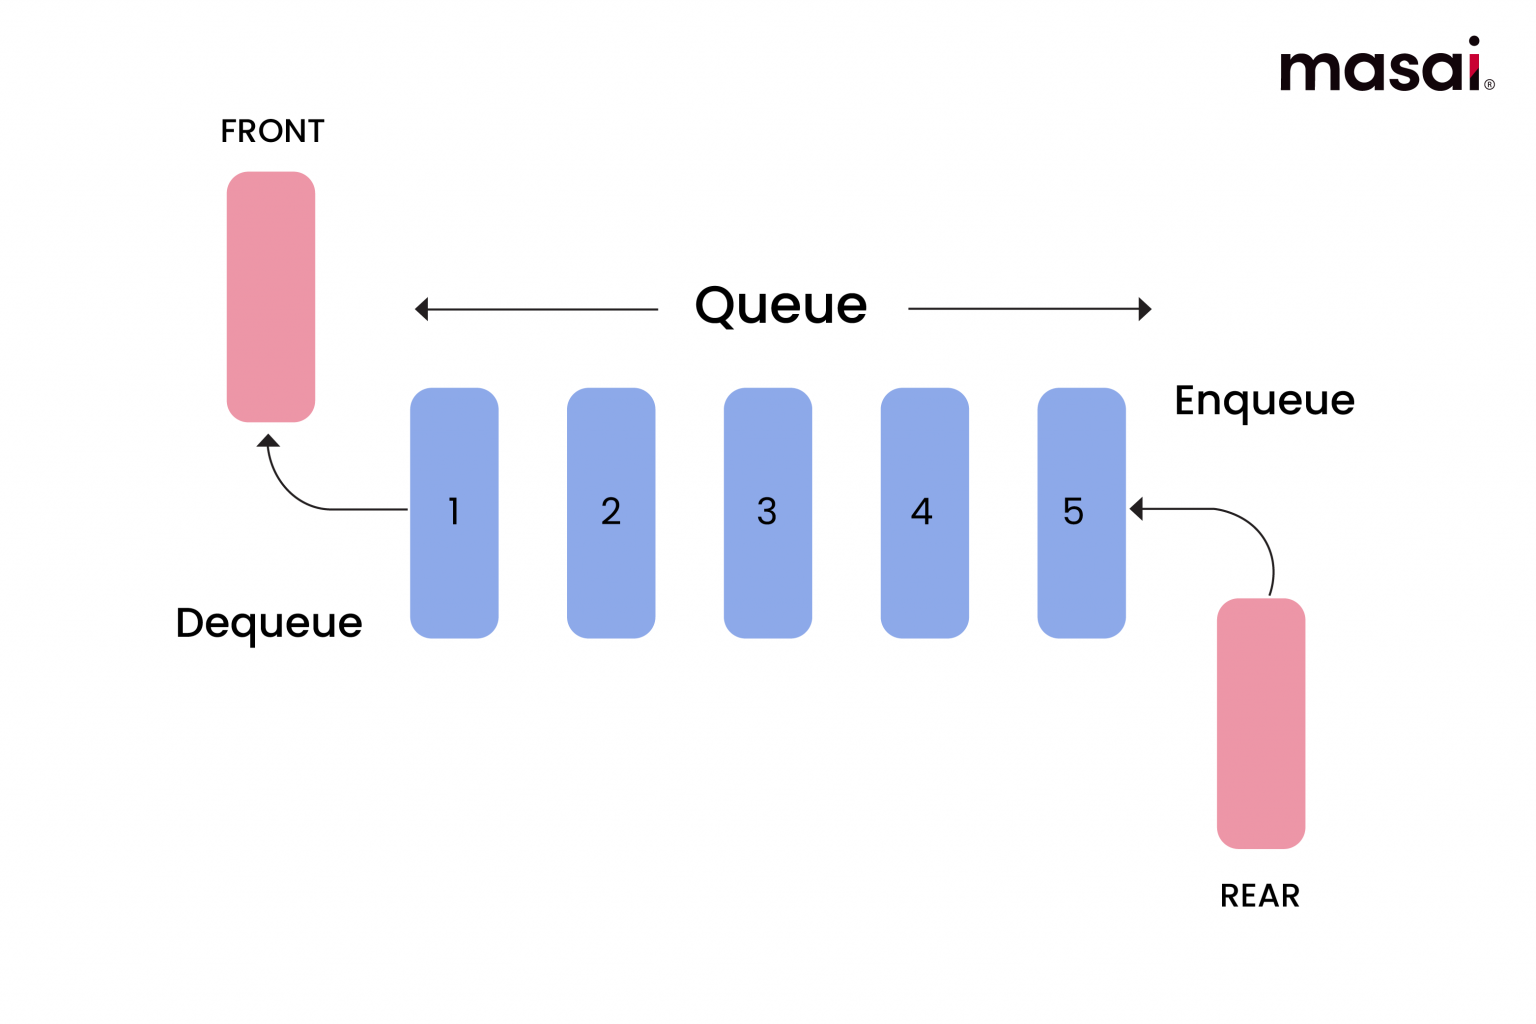
\includegraphics[width=0.9\textwidth]{resources/19-26/queue.png}

В стандартной библиотеке C++ присутствует \cppref[шаблон класса]{cpp/container/queue} \mverb{std::queue<T>}, который является оберткой поверх
какого-либо другого контейнера (по умолчанию, \cppref[\texttt{std::deque<T>}]{cpp/container/deque}).

\subsection{Операции над очередями}
Когда речь идет об очереди, подразумевается структура данных со следующими операциями:
\begin{enumerate}
  \item Добавить элемент в конец (хвост) очереди (\mverb{enqueue()}, в С++ \mverb{push()}).
  \item Удалить элемент из головы очереди (\mverb{dequeue()}, в C++ \mverb{pop()}).
  \item Найти элемент в очереди.
\end{enumerate}
%
Часто также требуется операция чтения головы (\mverb{front()}) и проверки на пустоту (\mverb{empty()}). В эффективной реализации
все указанные операции, кроме поиска, должны выполнятся за \(O(1)\). Поиск выполняется за $O(n)$.

\subsection{Реализация очереди}
Приведем реализацию очереди (С++ 11) на основе кольцевого буфера. Реализация использует шаблоны и \cppref[\texttt{assert(bool)}]{cpp/error/assert}
для проверки инвариантов. Также, в данной реализации запрещена перезапись старых данных~--- в этом случае срабатывает \mverb{assert(bool)} \footnote{Можно заметить, что в операциях с очередью над кольцевым буфером используется операция взятия остатка от деления. Это сравнительно
  медленная операция. Если размер очереди (беззнаковое целое) представляет собой степень \(2\), эту операцию можно заменить на побитовое И. Впрочем, современные
  компиляторы делают это автоматически.}.

\begin{minted}{C++}
template <typename T, size_t N> class Queue {
public:
  Queue() = default;
  ~Queue() = default;

  bool empty() const { return count_ == 0; }
  size_t capacity() const { return N; }
  size_t count() const { return count_; }

  T &Peek() {
    assert(count_ > 0 && "Queue is empty.");
    return data_[start_];
  }
  const T &Peek() const {
    assert(count_ > 0 && "Queue is empty.");
    return data_[start_];
  }

  void Enqueue(T &&item) {
    assert(count_ < N && "Queue is full.");
    data_[end_] = item;
    end_ = (end_ + 1) % N;
    ++count_;
  }
  void Enqueue(const T &item) {
    assert(count_ < N && "Queue is full.");
    data_[end_] = item;
    end_ = (end_ + 1) % N;
    ++count_;
  }

  T Dequeue() {
    assert(count_ > 0 && "Queue is empty.");
    T item = data_[start_];
    start_ = (start_ + 1) % N;
    --count_;
    return item;
  }

  T* Find(const T& item) {
    for (size_t i = 0; i < count_; ++i) {
      if (data_[(start_ + i) % N] == item) {
        return &data_[(start_ + i) % N];
      }
    }
    return nullptr;
  }

private:
  T data_[N];
  size_t start_{};
  size_t end_{};
  size_t count_{};
};
\end{minted}
